\documentclass[a4paper,12pt,titlepage,bibliography=numbered]{article}
\usepackage[margin=1in]{geometry}
\usepackage{graphicx} % Required for inserting images
\usepackage{amsmath}
\usepackage{float}
\begin{document}

\begin{figure}[H]
\centering
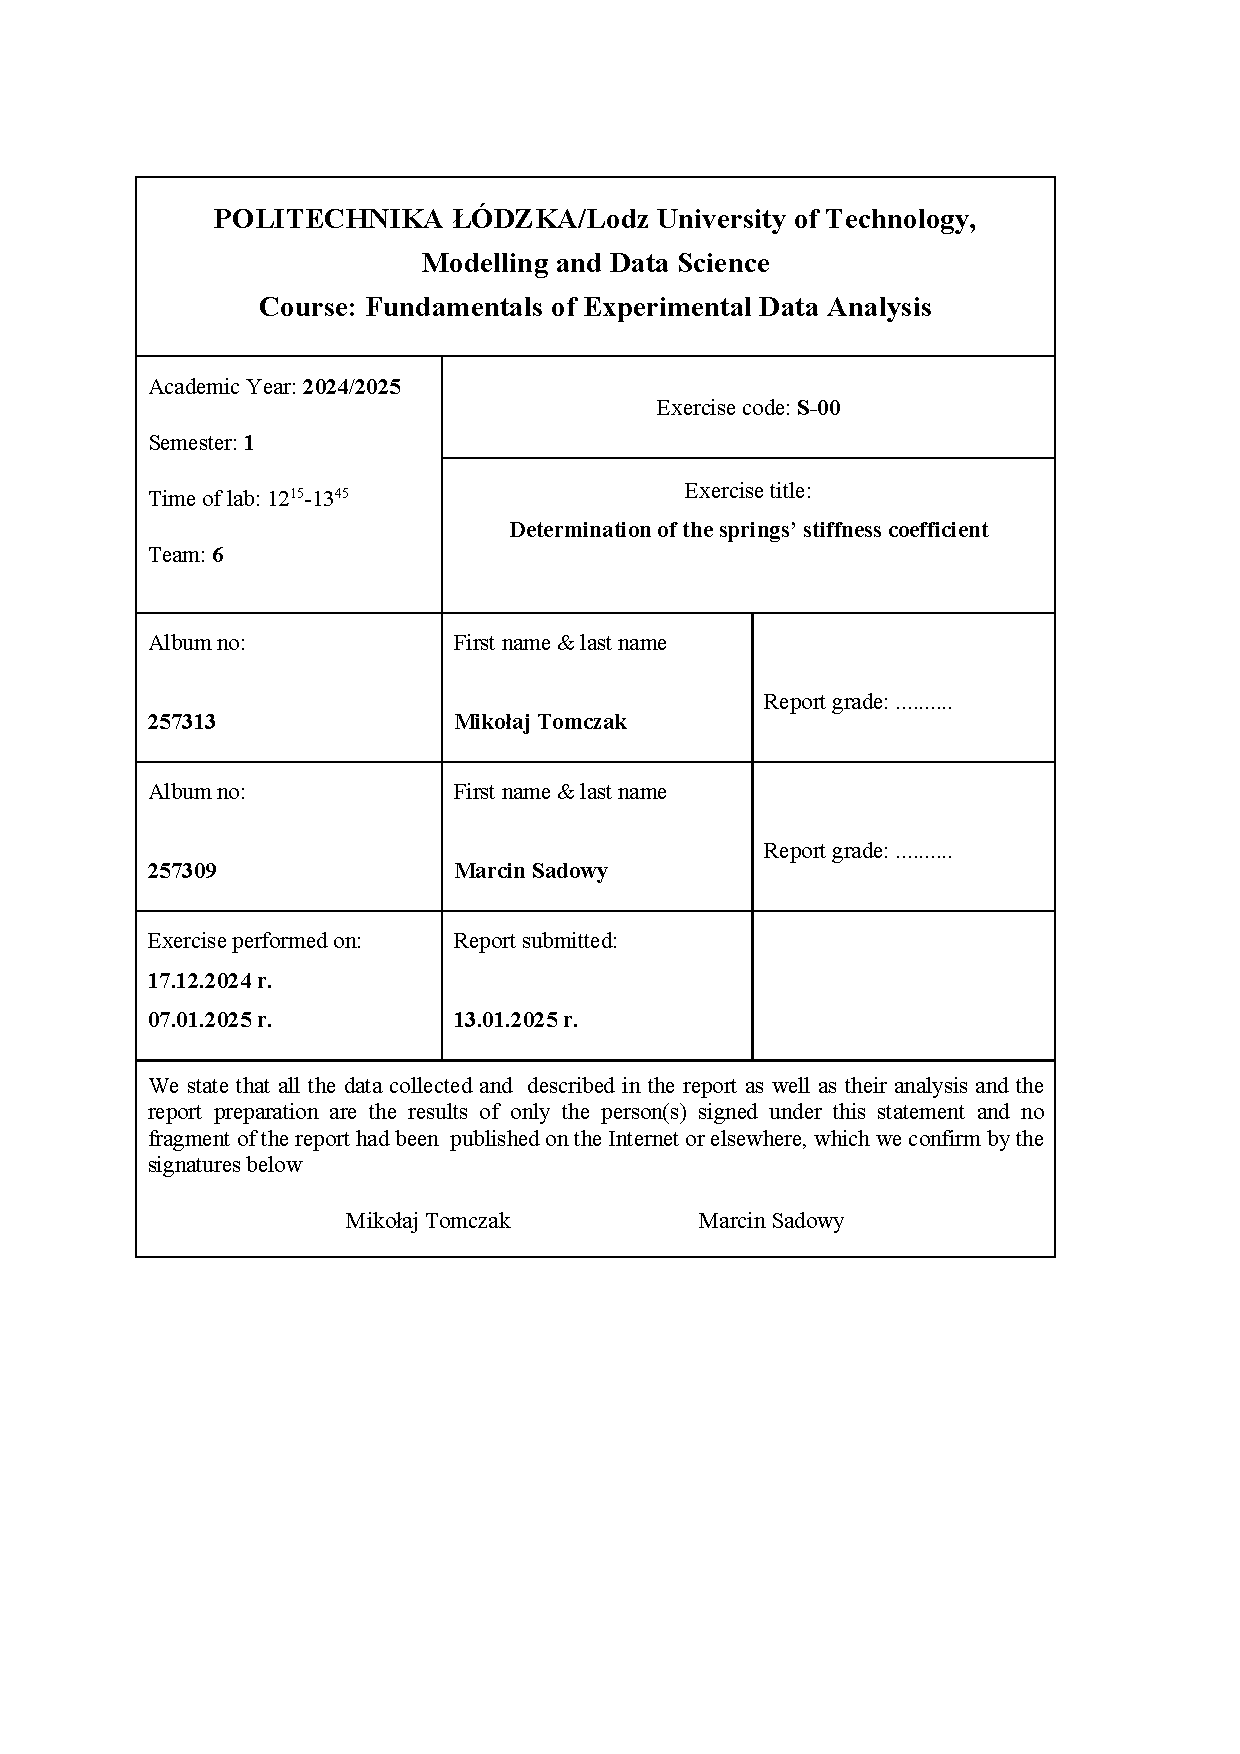
\includegraphics[width=1\textwidth]{first_page.pdf}
\end{figure}

\section{The aim of the experiment}

The aim of the experiment is [\ref{instruction}]:
\begin{enumerate}
\item Learning about the Hooke’s law and the oscillatory motion.
\item Learning and applying the linear least squares’ method.
\item Learning and applying methods of determining uncertainties in measurements.
\end{enumerate}

\section{Measurement Method}

We started by weighing each mass five times using a digital scale. To determine the spring constant $k$ and the equivalent stiffness $k_{eff}$ of system with series connected springs, we used the static method for both and the dynamic method for the spring constant $k$. For the static method, we measured the stiffness of the spring by attaching various weights of different masses $m$. We recorded the spring deformation for each weight combination using a meter, repeating each measurement five times. To determine $k$ using the static method, we relied on the principle that the gravitational force $Q$ acting on the spring is balanced by the spring's restoring force $F$.\\\\ 
By equating formulas:

\begin{equation}
    Q = mg,
    \label{Gravity}
\end{equation}
$Q$ - the gravitational force acting on the spring, $m$ - mass attached to one end of a spring hanging in the gravitational field, $g$ - Earths' gravity
\begin{equation}
    F = -kx.
    \label{Force}
\end{equation}
$F$ - force acting on the spring to restore it to its original form, $k$ - the stiffness of the spring, $x$ - the deformation of the spring\\\\
\noindent We obtain the following:

\begin{equation}
    k = \frac{mg}{x}. 
    \label{Force}
\end{equation}

\noindent We repeated the measurements for the springs connected in a series configuration.
The effective stiffness $k_{eff}$ was calculated using the following formula:

\begin{equation}
    \frac{1}{k_{eff}} = \sum_{i=1}^N \frac{1}{k_i}
    \label{effective_stiffness}
\end{equation}

\noindent In the dynamic method, we set the springs into oscillatory motion by attaching different combinations of weights of varying masses m and displacing them from their equilibrium position. Using a stopwatch, we recorded the time for 30 complete oscillations for each mass. The period T was calculated as the average time per oscillation. 
Using the formula for the period of oscillation:

\begin{equation}
    T = 2 \pi \sqrt{\frac{m}{k}}
\end{equation}

\noindent We rearranged and squared the equation to obtain:

\begin{equation}
    T^2 = \frac{4 \pi^2}{k}m
    \label{T_squered}
\end{equation}

\noindent By plotting $T^2$ versus $m$ and analyzing the slope of the resulting line using the linear least squares’ method, we calculated the stiffness $k$.

\section{Results of the measurements and calculations}

In table \ref{table_wth_weights} we collected the measured masses of 11 weights, and we also calculated their uncertainties from:

\begin{equation}
    u_A(x) = \sqrt{\frac{1}{n(n-1)}\sum_{i=1}^N(x_i-x)^2}
    \label{mass_uncertainty_A}
\end{equation}

\begin{equation}
    u_B(x) = \sqrt{\frac{(\Delta_p x)^2}{3} + \frac{(\Delta_e x)^2}{3}}
    \label{mass_uncertainty_B}
\end{equation}

\begin{equation}
    u(x) = \sqrt{u_A^2(x) + u_B^2(x)}
    \label{mass_uncertainty}
\end{equation}

\noindent \\The type A uncertainty differs depending on the measurement, but the type B uncertainty is constant and equal to: \\

\begin{equation}
    u_B(m) = \sqrt{\frac{(0.01 g)^2}{3} + \frac{(0.02 g)^2}{3}} = 0.012910 \mathrm{g} \\
\end{equation}

\begin{table}[H]
\centering
\caption{The measured masses of 11 weights with their uncertainties} \label{table_wth_weights}
\begin{tabular}{|c|c|c|c|c|c|c|}
\hline
Measurement Number & 1 & 2 & 3 & 4 & 5 & Mean \\ 
\hline
$m_1$ [g] & 99.88 & 99.87 & 99.87 & 99.89 & 99.88 & 99.876 \\ 
\hline
$m_2$ [g] & 100.89 & 100.9 & 100.89 & 100.9 & 100.89 & 100.892 \\ 
\hline
$m_3$ [g] & 100.88 & 100.88 & 100.88 & 100.89 & 100.89 & 100.886 \\ 
\hline
$m_4$ [g] & 100.25 & 100.26 & 100.25 & 100.25 & 100.25 & 100.252 \\ 
\hline
$m_5$ [g] & 100.49 & 100.5 & 100.5 & 100.49 & 100.48 & 100.492 \\ 
\hline
$m_6$ [g] & 49.86 & 49.86 & 49.87 & 49.75 & 49.76 & 49.82 \\
\hline
$m_7$ [g] & 49.75 & 49.75 & 49.76 & 49.75 & 49.76 & 49.754 \\ 
\hline
$m_8$ [g] & 49.97 & 49.98 & 49.98 & 49.97 & 49.97 & 49.976 \\ 
\hline
$m_9$ [g] & 9.98 & 9.98 & 9.99 & 9.98 & 9.98 & 9.982 \\
\hline
$m_{10}$ [g] & 9.99 & 9.99 & 9.99 & 9.98 & 9.98 & 9.988 \\ 
\hline
$m_{11}$ [g] & 19.86 & 19.87 & 19.86 & 19.86 & 19.87 & 19.864 \\ 
\hline
$u_A$(m) & 0.002191 & 0.001789 & 0.003578 & 0.001789 & 0.003347 & --- \\ 
\hline
$u(m)$ & 0.02012 & 0.02008 & 0.02317 & 0.02008 & 0.020278 & --- \\ 
\hline
\end{tabular}
\end{table}

\noindent Table 2 shows the results of the deformation measurement for the first spring. Once again we calculated the uncertainties of the deformation using Eqs. (\ref{mass_uncertainty_A}),(\ref{mass_uncertainty_B}) and (\ref{mass_uncertainty}).
\begin{table}[H]
\centering
\caption{The results of the deformation measurement for the first spring with uncertainties.} \label{table_wth_deformation_1}
\begin{tabular}{|c|c|c|c|c|c|c|c|c|c|c|}
\hline
\textbf{-} & \textbf{1 [cm]} & \textbf{2 [cm]} & \textbf{3 [cm]} & \textbf{4 [cm]} & \textbf{5 [cm]}& \textbf{Mean [cm]} & \textbf{$u_A(x)$} & \textbf{$u(x)$} \\ 
\hline
$m_1 - m_{11}$ & 28.4 & 28.4 & 28.2 & 28.1 & 28.0 & 28.22 & 0.071554 & 0.072709 \\ 
\hline
$m_1 - m_{10}$ & 27.4 & 27.2 & 27.2 & 27.2 & 27.1 & 27,22 & 0.043818 & 0.04568 \\ 
\hline
$m_1 - m_8$ & 26.6 & 26.7 & 26.8 & 26.7 & 26.9 & 26,74 & 0.045607 & 0.047399 \\ 
\hline
$m_1 - m_6$ & 22.7 & 22.6 & 22.7 & 22.7 & 22.8 & 22,7 & 0.028284 & 0.031091 \\ 
\hline
$m_1 - m_5$ & 20.7 & 20.8 & 20.9 & 20.6 & 20.8 & 20,76 & 0.045607 & 0.047399 \\ 
\hline
$m_1 - m_4$ & 16.8 & 16.9 & 16.9 & 16.7 & 16.7 & 16,8 & 0.04 & 0.042032 \\ 
\hline
$m_1 - m_3$ & 12.7 & 12.5 & 12.6 & 12.7 & 12.8 & 12,66 & 0.045607 & 0.047399 \\ 
\hline
$m_1 - m_2$ & 8.3 & 8.5 & 8.5 & 8.4 & 8.4 & 8,42 & 0.033466 & 0.03587 \\ 
\hline
\end{tabular}
\end{table}

\noindent The type B uncertainty is once again constant and equal to: \\
\begin{equation}
    u_B(x) = \sqrt{\frac{(0.01 \mathrm{mm})^2}{3} + \frac{(0.02 \mathrm{mm})^2}{3}} = 0.012910 \mathrm{mm}
\end{equation}

\noindent \\This quantity stays the same in the measurement of the deformation of the second spring and of the springs connected in series, so we will not repeat it. The notation \(m_i - m_j\) indicates the sum of the masses from index i to index j. We can determine the formula for the stiffness coefficient \(k\) from:
\begin{equation}
    x = \frac{mg}{k}
\end{equation}
Therefore, the stiffness coefficient can be obtained by calculating the slope coefficient of the $x(m)$ function.
\begin{figure}[H]
\centering
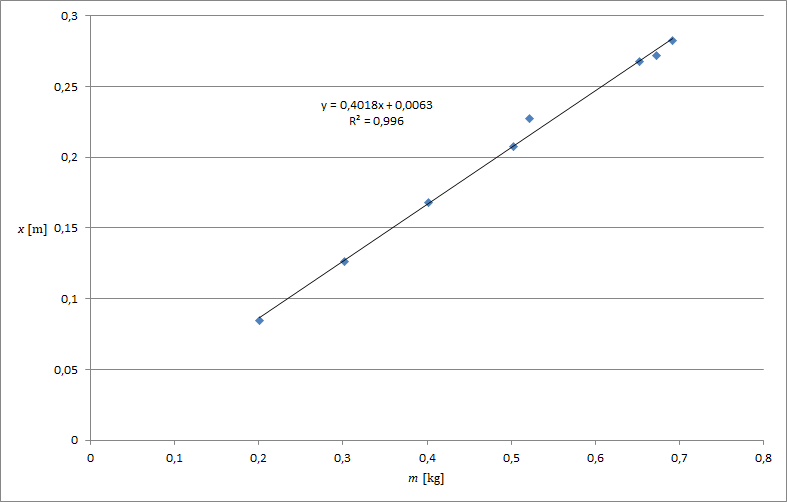
\includegraphics[width=1\textwidth]{fig1.png}
\caption{The dependence of the deformation of the first spring on the mass.}
\label{fig_1}
\end{figure}
\begin{equation}
    a_1 = 0.401 \mathrm{\frac{m}{kg}}
\end{equation}
We can then solve for $k$ by dividing the slope coefficient by the acceleration due to Earth's gravity. \\
\begin{equation}
    k = \frac{g}{a}
    \label{slope_to_stiffness}
\end{equation}
So, the stiffness coefficient of the first spring is: 
\begin{equation}
    k_1 = \frac{9.81}{0.401} = 24.525 \mathrm{\frac{kg}{s^2}}
\end{equation}
\noindent Table 3 shows the result of the deformation measurements for the second spring. Once again we calculated the uncertainties of the deformation using Eqs. (\ref{mass_uncertainty_A}),(\ref{mass_uncertainty_B}) and (\ref{mass_uncertainty}).
\noindent The type B uncertainty is once again constant and equal to: \\
\begin{equation}
    u_B(x) = \sqrt{\frac{(0.01 \mathrm{mm})^2}{3} + \frac{(0.02 \mathrm{mm})^2}{3}} = 0.012910 \mathrm{mm}
\end{equation}

\begin{table}[H]
\centering
\caption{The results of the deformation measurement for the second spring.}
\begin{tabular}{|c|c|c|c|c|c|c|c|c|}
\hline
\textbf{-} & \textbf{1 [cm]} & \textbf{2 [cm]} & \textbf{3 [cm]} & \textbf{4 [cm]} & \textbf{5 [cm]} & \textbf{Mean [cm]} & \textbf{$u_A$(x)} & \textbf{$u(x)$} \\ 
\hline
$m_1 - m_{11}$ & 26.5 & 26.6 & 26.5 & 26.5 & 26.4 & 26.5 & 0.028284 & 0.031091 \\ 
\hline
$m_1 - m_{10}$ & 25.8 & 25.7 & 25.7 & 25.7 & 25.6 & 25.7 & 0.028284 & 0.031091 \\ 
\hline
$m_1 - m_8$ & 25.1 & 24.7 & 24.8 & 24.9 & 24.9 & 24.88 & 0.05933 & 0.060718 \\ 
\hline
$m_1 - m_6$ & 20.8 & 20.7 & 20.8 & 20.9 & 21.0 & 20.84 & 0.045607 & 0.047399 \\ 
\hline
$m_1 - m_5$ & 18.8 & 19.0 & 18.9 & 18.9 & 18.9 & 18.92 & 0.033466 & 0.03587 \\ 
\hline
$m_1 - m_4$ & 15.1 & 15.0 & 15.0 & 15.1 & 15.2 & 15.08 & 0.033466 & 0.03587 \\ 
\hline
$m_1 - m_3$ & 10.9 & 11.0 & 11.0 & 10.9 & 10.9 & 10.96 & 0.021909 & 0.02543 \\ 
\hline
$m_1 - m_2$ & 7.9 & 7.2 & 7.2 & 7.1 & 7.2 & 7.32 & 0.130843 & 0.131479 \\ 
\hline
\end{tabular}
\end{table}

\begin{figure}[H]
\centering
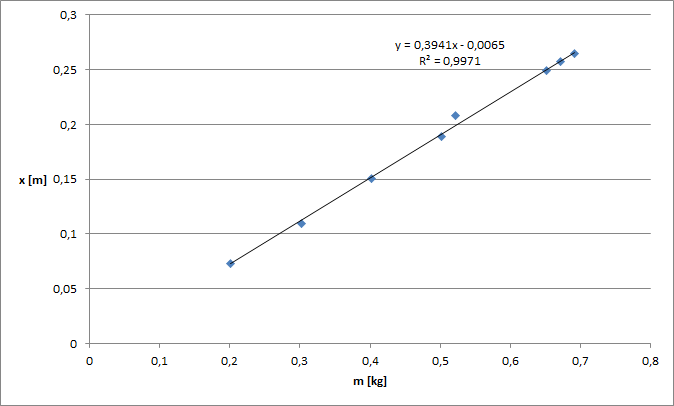
\includegraphics[width=1\textwidth]{fig2.png}
\caption{The dependence of the deformation of the first spring on the mass.}
\label{fig_2}
\end{figure}
\noindent We can see that the slope coefficient of the function is equal to
\begin{equation}
    a_2 = 0.394 \mathrm{\frac{m}{kg}}.
\end{equation}

Using Eq. (\ref{slope_to_stiffness}) we can calculate the stiffness coefficient of the second spring: \\
\begin{equation}
    k_2 = \frac{9.81}{0.394} = 24.898 \mathrm{\frac{kg}{s^2}}
\end{equation}

\begin{table}[H]
\centering
\caption{The results of the deformation measurement for the system of two springs connected in series.}
\begin{tabular}{|c|c|c|c|c|c|c|c|c|c|}
\hline
\textbf{-} & \textbf{1 [cm]} & \textbf{2 [cm]} & \textbf{3 [cm]} & \textbf{4 [cm]} & \textbf{5 [cm]} & \textbf{Mean} & \textbf{$u_A(x)$} & \textbf{$u(x)$} \\ 
\hline
$m_1 - m_1$ & 25.7 & 25.9 & 25.7 & 25.8 & 25.9 & 25.8 & 0.04 & 0.042032 \\ 
\hline
$m_1 - m_2$ & 33.9 & 34.2 & 34.0 & 34.0 & 34.2 & 34.06 & 0.053666 & 0.055197 \\ 
\hline
$m_1 - m_3$ & 42.1 & 42.2 & 42.3 & 42.3 & 42.3 & 42.2 & 0.04 & 0.042032 \\ 
\hline
$m_1 - m_4$ & 50.4 & 50.4 & 50.4 & 50.3 & 50.4 & 50.38 & 0.017889 & 0.022061 \\ 
\hline
$m_1 - m_5$ & 58.3 & 58.5 & 58.4 & 58.3 & 58.5 & 58.4 & 0.04 & 0.042032 \\ 
\hline
$m_1 - m_6$ & 59.4 & 59.6 & 59.5 & 59.4 & 59.6 & 59.5 & 0.04 & 0.042032 \\ 
\hline
$m_1 - m_7$ & 62.8 & 63.0 & 63.2 & 63.2 & 63.2 & 63.06 & 0.066933 & 0.068166 \\ 
\hline
$m_1 - m_8$ & 66.8 & 66.9 & 66.8 & 66.8 & 66.7 & 66.8 & 0.028284 & 0.031091 \\ 
\hline
\end{tabular}
\end{table}
\begin{figure}[H]
\centering
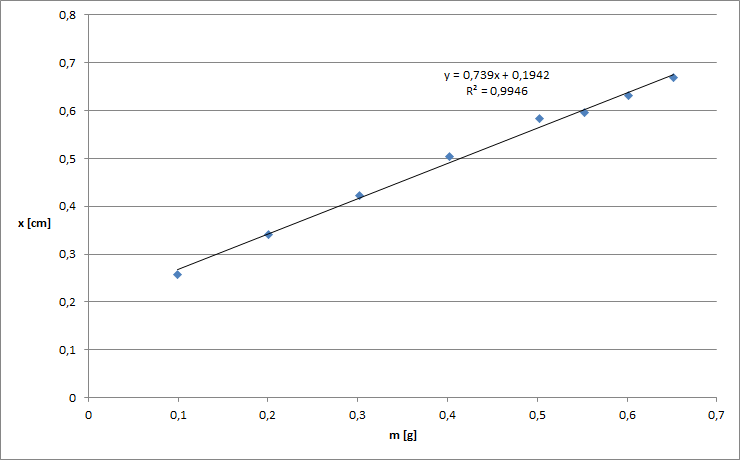
\includegraphics[width=1\textwidth]{fig3.png}
\caption{The dependence of the deformation of the spring system on the mass.}
\label{fig_3}
\end{figure}
\noindent The slope coefficient is equal to
\begin{equation}
    a_3 = 0.739 \mathrm{\frac{m}{kg}}.
\end{equation}
Once again we derive the stiffness coefficient of the system of springs using Eq. (\ref{slope_to_stiffness}): \\ 
\begin{equation}
    k_3 = \frac{9.81}{0.739}  = 13.275 \mathrm{\frac{kg}{s^2}}
    \label{k_3}
\end{equation}
The result is close to the one that can be derived using Eq (7). If we solve for \(k_{eff}\) we obtain that:
\begin{equation}
    k_{eff} = \frac{k_1 \cdot k_2}{k_1 + k_2}
\end{equation}
So, in this case
\begin{equation}
    k_3 = \frac{k_1 \cdot k_2}{k_1 + k_2} = \frac{24.525 \times 24.898}{24.525+24.898} = 12.355 \mathrm{\frac{kg}{s^2}}
\end{equation}
The result is close to the one obtained from the slope coefficient. \\
Then we calculate the stiffness coefficient of the second spring using the dynamic method. Table 5 shows the result of the measurement of 30 oscillations for different masses. The table also includes the period, type A uncertainty, as well as the standard combined uncertainty of each time measurement, which are obtained from Eqs. (\ref{mass_uncertainty_A}) and (\ref{mass_uncertainty}). The type B uncertainty is not in the table as it is constant and can be calculated by using Eq. (\ref{mass_uncertainty_B}): \\
\begin{equation}
    u_B(t) = \sqrt{\frac{(0.01 s)^2}{3} + \frac{(0.5 s)^2}{3}} = 0.28873 \mathrm{s}
\end{equation}
\begin{figure}[H]
\centering
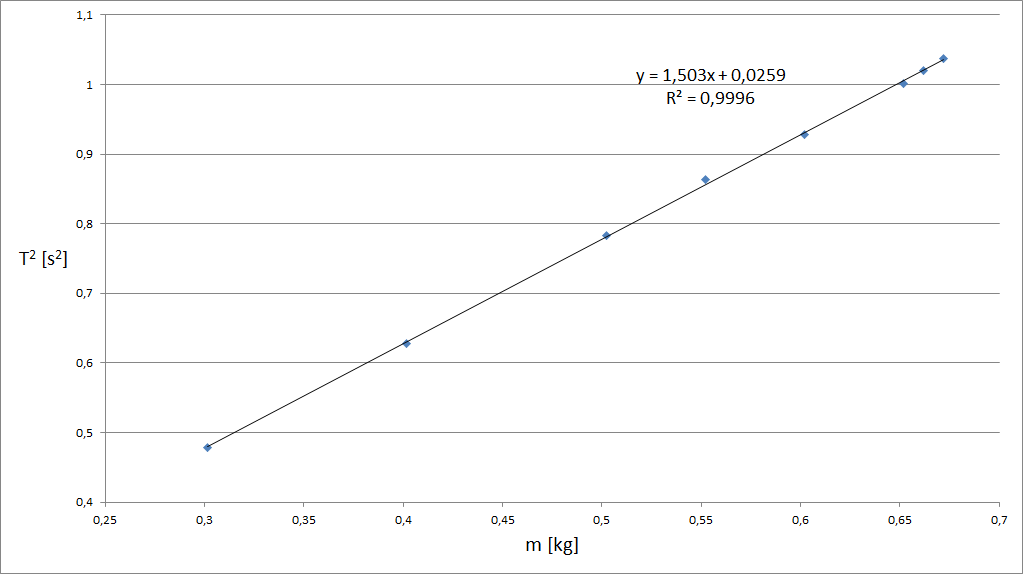
\includegraphics[width=1\textwidth]{fig4.png}
\caption{The dependence of the square of the period on the mass.}
\label{fig_4}
\end{figure}
\noindent From Eq. (\ref{T_squered}) we can observe that the slope coefficient of the dependence is equal to
\begin{equation}
a = \frac{4 \pi ^2}{k}.    
\end{equation}
By solving for k we arrive at the equation:
\begin{equation}
    k = \frac{4 \pi ^2}{a}
    \label{k_with_pi}
\end{equation}
We can observe on the figure that the slope coefficient of the function is: \(a_4 = 1.503 \mathrm{\frac{s^2}{kg}}\) \\ 
We then calculate the spring coefficient k of the second spring using Eq. (\ref{T_squered}): \\
\begin{equation}
    k_4 = \frac{4 \pi ^2}{1.503} = 26.266 \mathrm{\frac{kg}{s^2}}
\end{equation}
We can observe that the obtained coefficient is close in value to \(k_1\), which is equal to \(24.898 \mathrm{\frac{kg}{s^2}}\). The difference is affected mainly by the time uncertainty of each measurement.\\\\
Now we can focus on calculation of the uncertainties of obtained stiffness coefficient. In the static method, where the stiffness coefficient is expressed by Eq. (\ref{slope_to_stiffness}), we can calculate $u(k)$ using propagation of uncertainty. \\
We define the sensitivity coefficients:
\begin{equation}
    c_g = \frac{1}{a}
\end{equation}
\begin{equation}
    c_a = -\frac{g}{a^2}
\end{equation}
For the calculations we use the uncertainty of g \(u(g) = 0.01 \mathrm{\frac{m}{s^2}}\). The uncertainty of the slope coefficients was obtained using the LINEST function in Microsoft Excel.
\begin{table}[H]
\centering
\caption{Summary results of measurement uncertainty values for the deformation measurement of the first spring}
\begin{tabular}{|c|c|c|c|}
\hline
\textbf{\(x_j\)} & \textbf{\(c_{x_j}\)} & \textbf{\(u(x_j)\)} \\ \hline
\(g \mathrm{\frac{m}{s^2}}\) & 2.4938 \(\mathrm{\frac{kg}{m}}\) & 0.01 \(\mathrm{\frac{m}{s^2}}\) \\ \hline
\(a \mathrm{\frac{m}{kg}}\) & -61.007 \(\mathrm{\frac{kg^2}{s^2 \cdot m}}\) & 0.004977 \(\mathrm{\frac{m}{kg}}\) \\ \hline
\end{tabular}
\end{table}
\noindent We then repeat the same calculations for the measurements of the deformations of the second spring, as well as the series of two springs connected in series. \\ 
Table \ref{secound_spring_table_uncertainties} shows the values of the sensitivity coefficients and the uncertainties used to determine the uncertainty of the stiffness coefficient for the measurement of the deformation of the second spring. \\
\begin{table}[H]
\centering
\caption{Summary results of measurement uncertainty values for the deformation measurement of the second spring}\label{secound_spring_table_uncertainties}
\begin{tabular}{|c|c|c|c|}
\hline
\textbf{\(x_j\)} & \textbf{\(c_{x_j}\)} & \textbf{\(u(x_j)\)} \\ \hline
\(g \mathrm{\frac{m}{s^2}}\) & 2.5381 \(\mathrm{\frac{kg}{m}}\) & 0.01 \(\mathrm{\frac{m}{s^2}}\) \\ \hline
\(a \mathrm{\frac{m}{kg}}\) & -63.194 \(\mathrm{\frac{kg^2}{s^2 \cdot m}}\) & 0.00414 \(\mathrm{\frac{m}{kg}}\) \\ \hline
\end{tabular}
\end{table}
\noindent Table \ref{system_spring_table_uncertainties} shows the values of the sensitivity coefficients and the uncertainties used to determine the uncertainty of the stiffness coefficient for the measurement of the deformation of the system of two springs connected in series.
\begin{table}[H]
\centering
\caption{Summary results of measurement uncertainty values for the deformation measurement of the system of two springs connected in series} \label{system_spring_table_uncertainties}
\begin{tabular}{|c|c|c|c|}
\hline
\textbf{\(x_j\)} & \textbf{\(c_{x_j}\)} & \textbf{\(u(x_j)\)} \\ \hline
\(g \mathrm{\frac{m}{s^2}}\) & 1.3532 \(\mathrm{\frac{kg}{m}}\) & 0.01 \(\mathrm{\frac{m}{s^2}}\) \\ \hline
\(a \mathrm{\frac{m}{kg}}\) & -17.963 \(\mathrm{\frac{kg^2}{s^2 \cdot m}}\) & 0.011677 \(\mathrm{\frac{m}{kg}}\) \\ \hline
\end{tabular}
\end{table}
\noindent The formula for the uncertainty of the stiffness coefficient is:
\begin{equation}
    u(k) = \sqrt{c_g^2u^2(g) + c_a^2u^2(a)}
    \label{u(k)_eq}
\end{equation}
Now we can determine the combined uncertainties of the stiffness coefficients of the first spring, the second spring, and the system of two springs connected in series. \\
\begin{equation}
    u_c(k_1) = \sqrt{2.4938^2 \times 0.01^2 + (-61.007)^2 \times 0.004977^2} = 0.30465 \mathrm{\frac{kg}{s^2}}
\end{equation}
\begin{equation}
    u_c(k_2) = \sqrt{2.5381^2 \times 0.01^2 + (-63.194)^2 \times 0.00414^2} = 0.26285 \mathrm{\frac{kg}{s^2}}
\end{equation}
\begin{equation}
    u_c(k_3) = \sqrt{1.3532^2 \times 0.01^2 + (-17.963)^2 \times 0.011677^2} = 0.21019 \mathrm{\frac{kg}{s^2}}
\end{equation}
When it comes to the dynamic method, we also use propagation of uncertainty, but for Eq. (\ref{k_with_pi}) \\
The sensitivity coefficient is:
\begin{equation}
    c_a = -\frac{4 \pi ^2 }{a^2}
\end{equation}
We calculate the uncertainty of the spring coefficient of the dynamic method using Eq. (\ref{u(k)_eq}).
\begin{equation}
    u_c(k_4) = \sqrt{(-\frac{4 \pi ^2}{1.503^2})^2 \times 0.004159^2} = 0.072683 \mathrm{\frac{kg}{s^2}}
\end{equation}
We can now calculate the expanded uncertainties of the stiffness coefficients for each measurement. We will be using the formula:
\begin{equation}
    U(k) = k \cdot u_c(k) = 2 \cdot u_c(k)
\end{equation}
We calculate:
\begin{equation}
    U(k_1) = 2 \times 0.30465 = 0.60930 \mathrm{\frac{kg}{s^2}}
\end{equation}
\begin{equation}
    U(k_2) = 2 \times 0.26285 = 0.52570 \mathrm{\frac{kg}{s^2}}
\end{equation}
\begin{equation}
    U(k_3) = 2 \times 0.21019 = 0.42038 \mathrm{\frac{kg}{s^2}}
\end{equation}
\begin{equation}
    U(k_4) = 2 \times 0.072683 = 0.145366 \mathrm{\frac{kg}{s^2}}
\end{equation}
\section{Results}
Finally we arrive at the obtained stiffness coefficients and their uncertainties:
\begin{equation}
    k_1 = 25(0.30) \mathrm{\frac{kg}{s^2}}, k_1 = (25 \pm 0.61) \mathrm{\frac{kg}{s^2}}
\end{equation}
\begin{equation}
    k_2 = 25(0.26) \mathrm{\frac{kg}{s^2}}, k_1 = (25 \pm 0.53) \mathrm{\frac{kg}{s^2}}
\end{equation}
\begin{equation}
    k_3 = 12(0.21) \mathrm{\frac{kg}{s^2}}, k_1 = (12 \pm 0.42) \mathrm{\frac{kg}{s^2}}
\end{equation}
\begin{equation}
    k_4 = 26(0.072) \mathrm{\frac{kg}{s^2}}, k_1 = (26 \pm 0.15) \mathrm{\frac{kg}{s^2}}
\end{equation}
The stiffness coefficient obtained from the dynamic method has substantially lower uncertainties than the stiffness coefficients obtained from the static method, which shows its superior precision.

\section{Conclusion}
\section{References}
\begin{enumerate}
    \item https://ftims.edu.p.lodz.pl/mod/resource/view.php?id=120359 \label{instruction}
\end{enumerate}
\section{Our Notes}
\begin{figure}
    \centering
    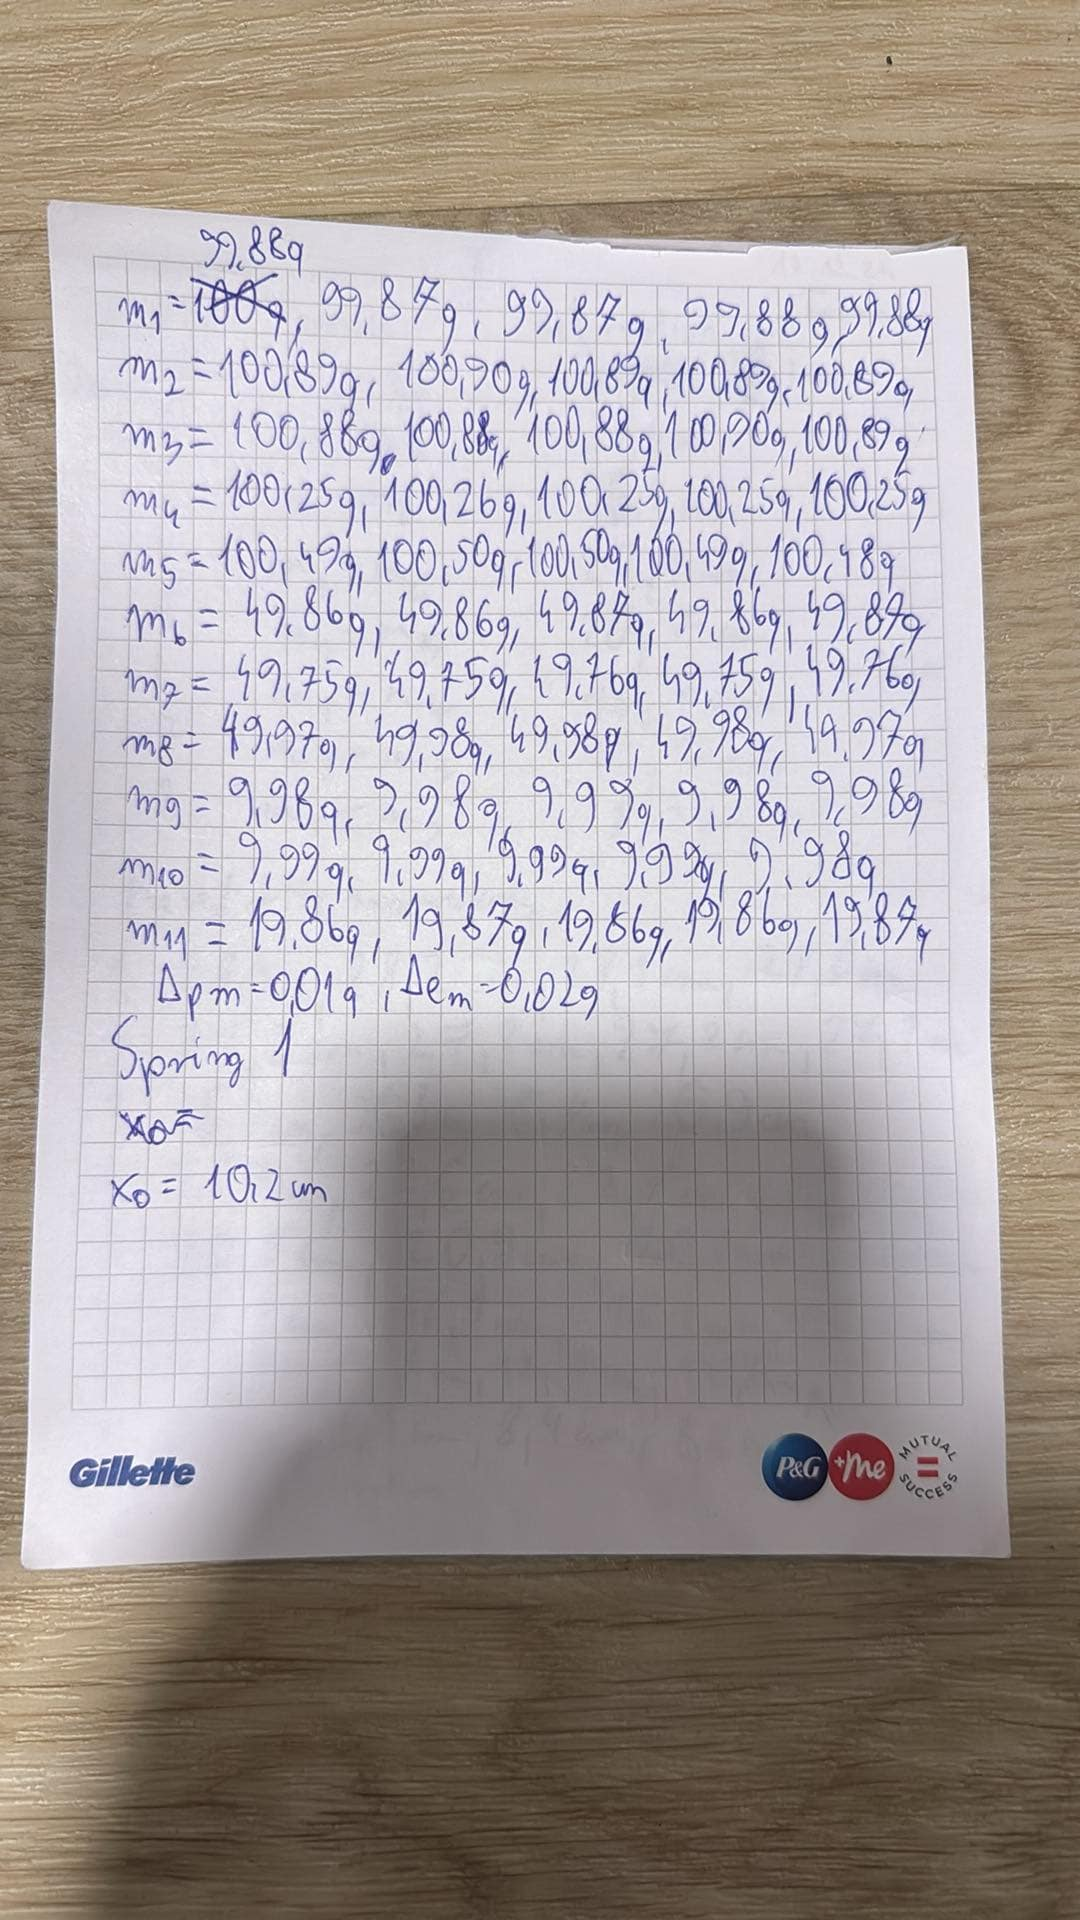
\includegraphics[width=0.5\linewidth]{notes1.jpeg}
\end{figure}
\begin{figure}
    \centering
    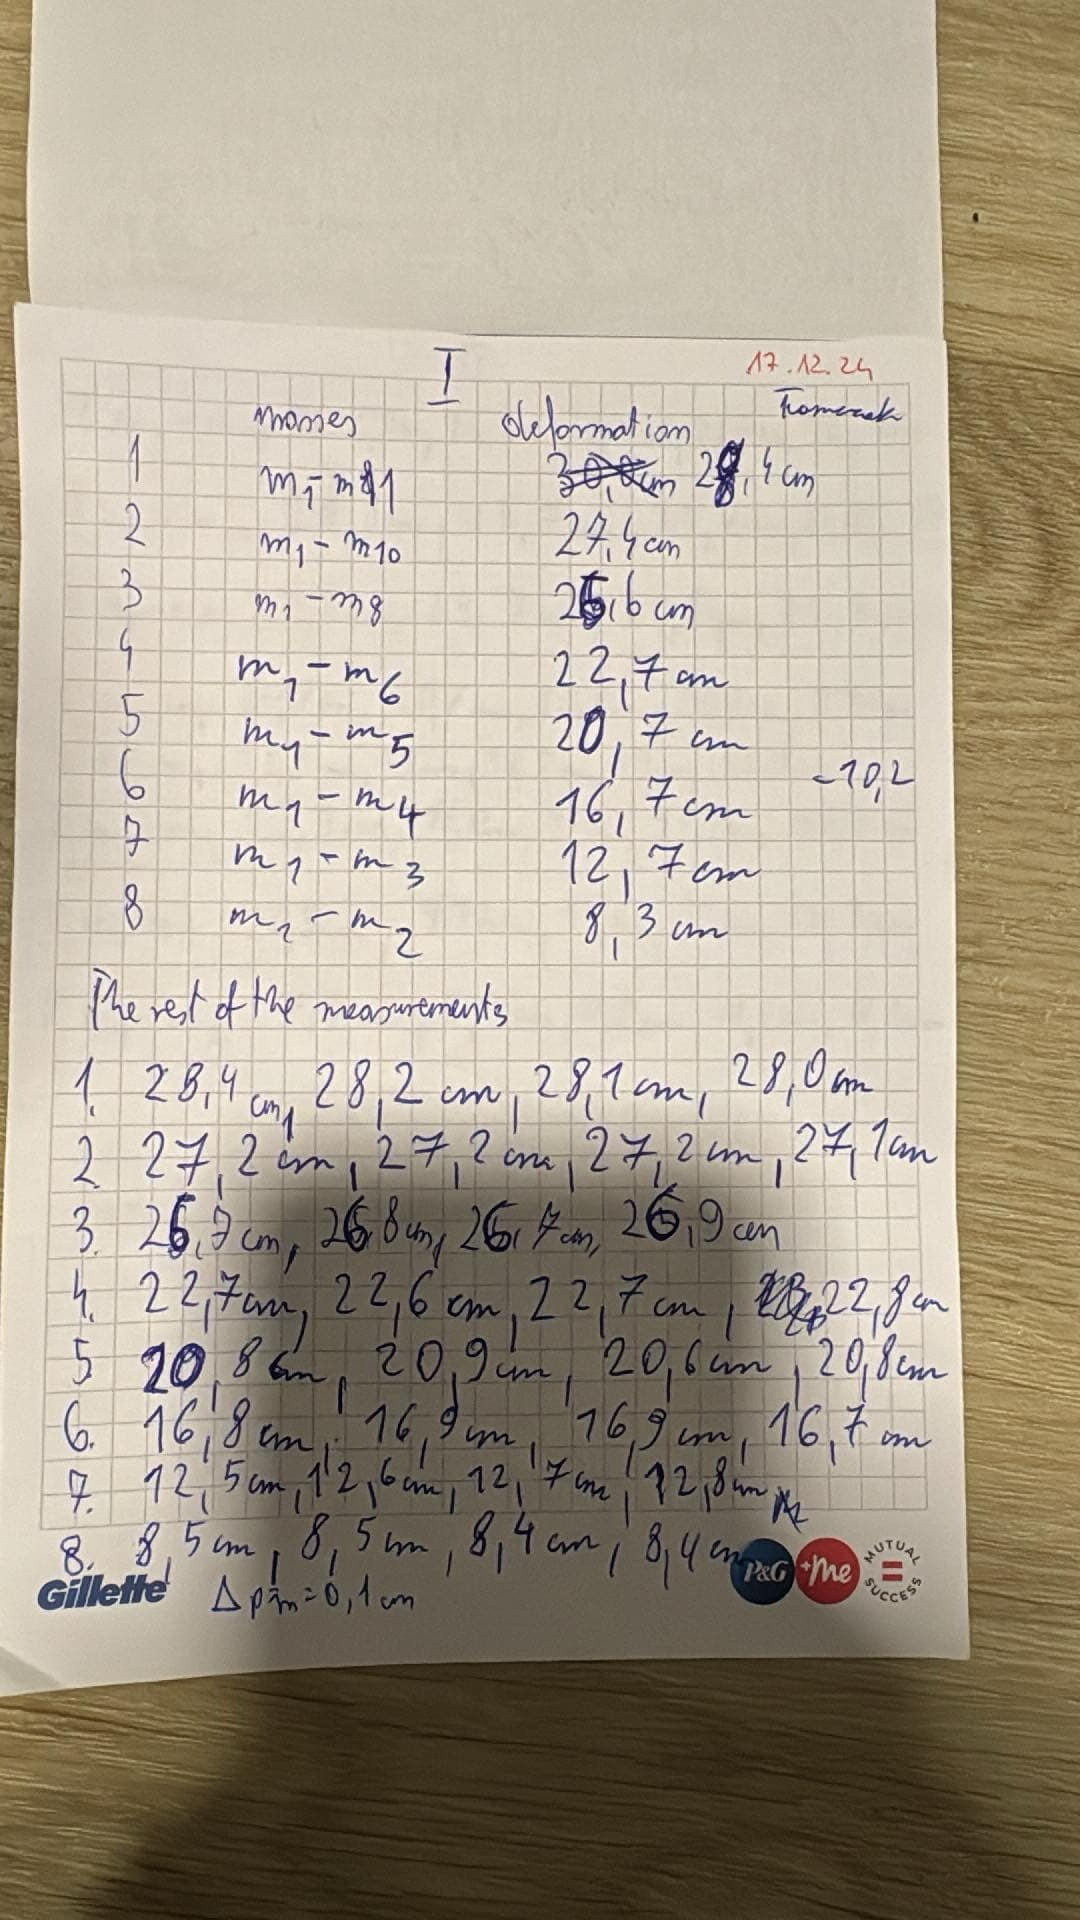
\includegraphics[width=0.5\linewidth]{notes2.jpeg}
\end{figure}
\begin{figure}
    \centering
    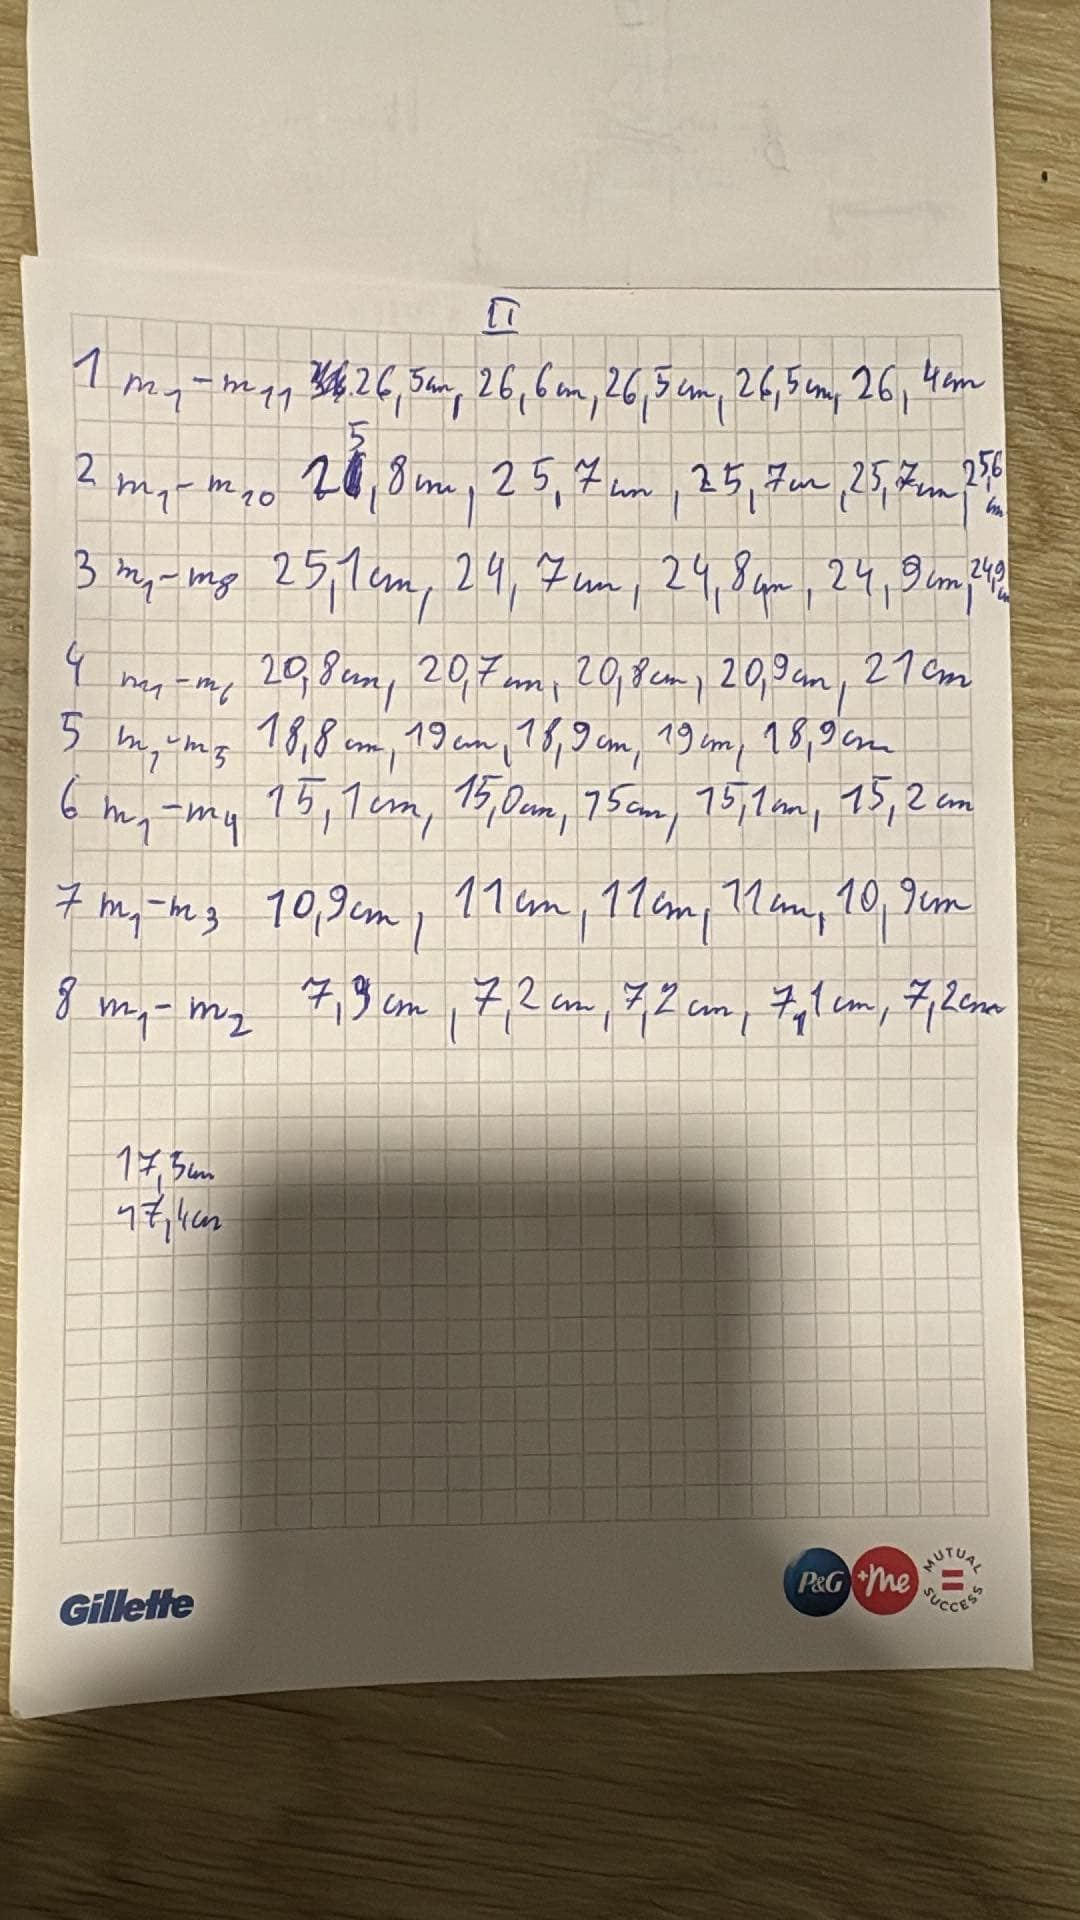
\includegraphics[width=0.5\linewidth]{notes3.jpeg}
\end{figure}
\begin{figure}
    \centering
    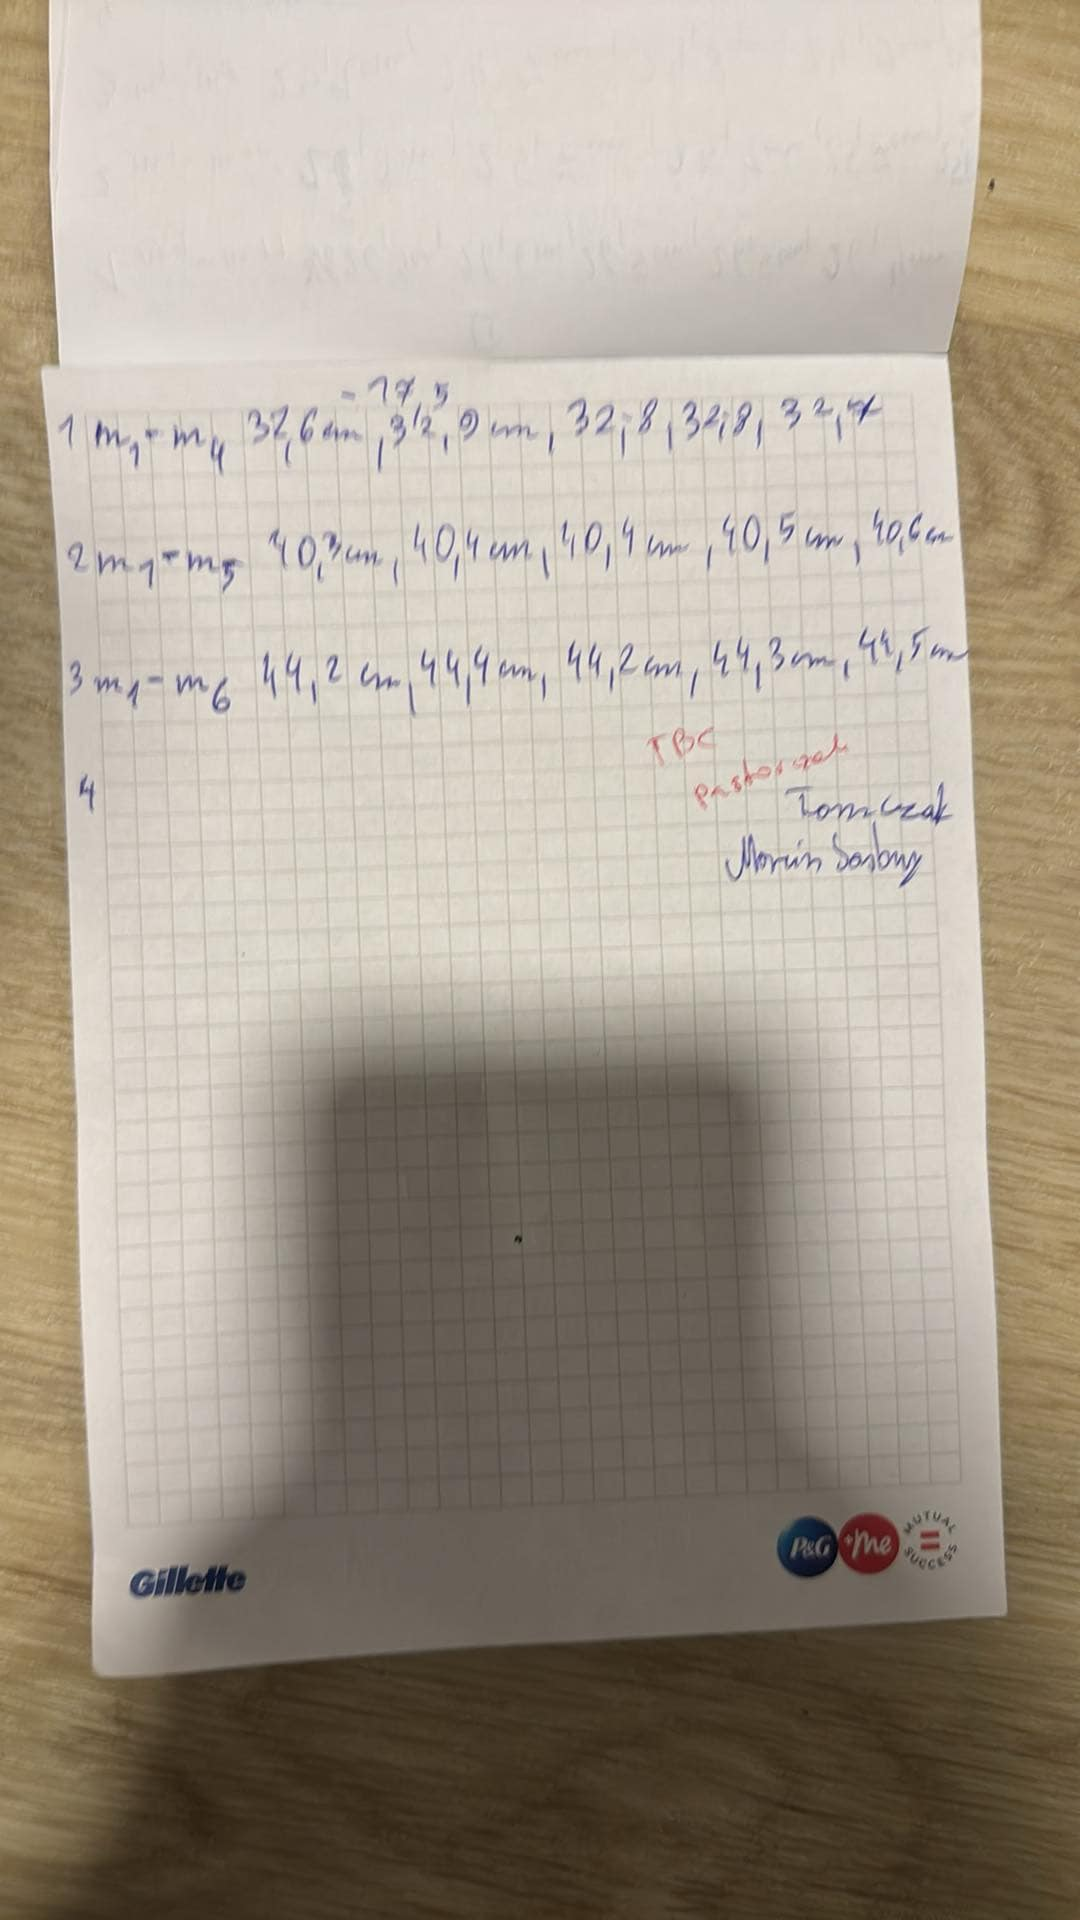
\includegraphics[width=0.5\linewidth]{notes4.jpeg}
\end{figure}
\begin{figure}
    \centering
    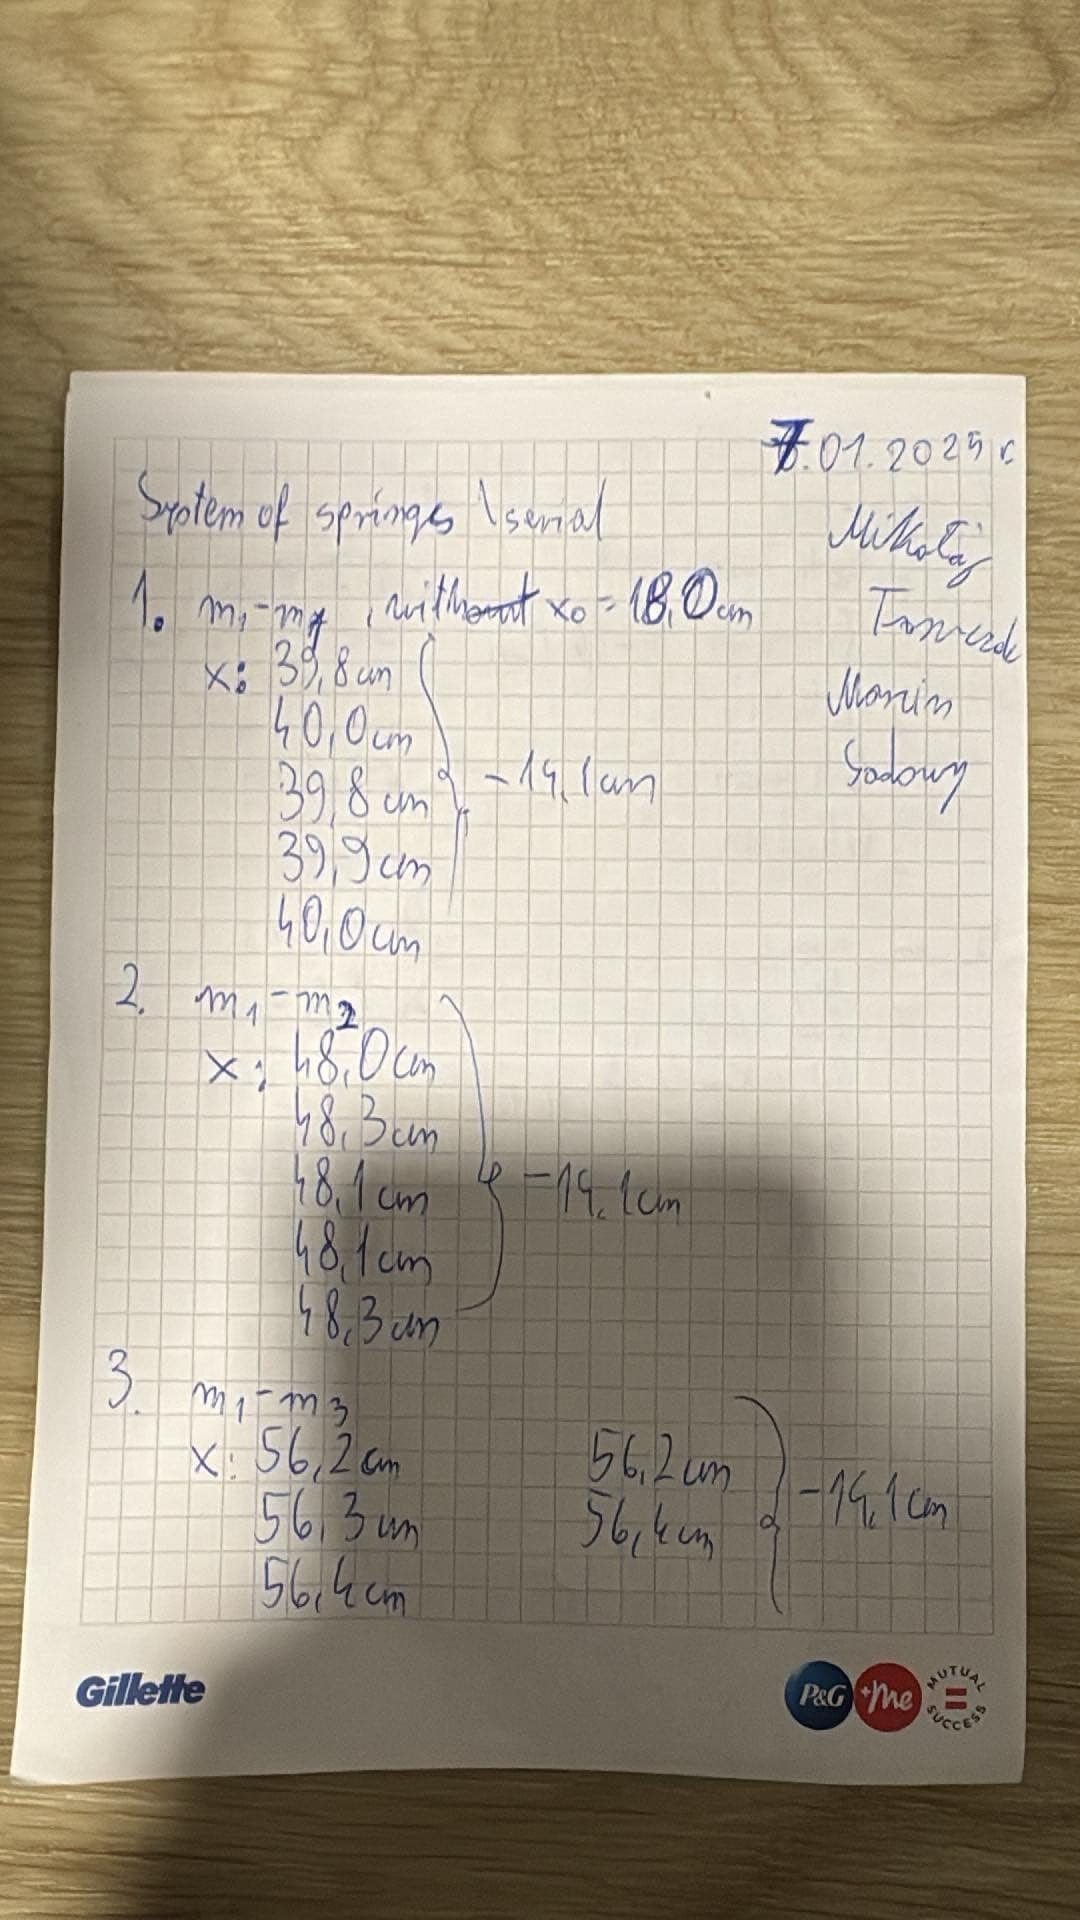
\includegraphics[width=0.5\linewidth]{notes5.jpeg}
\end{figure}
\begin{figure}
    \centering
    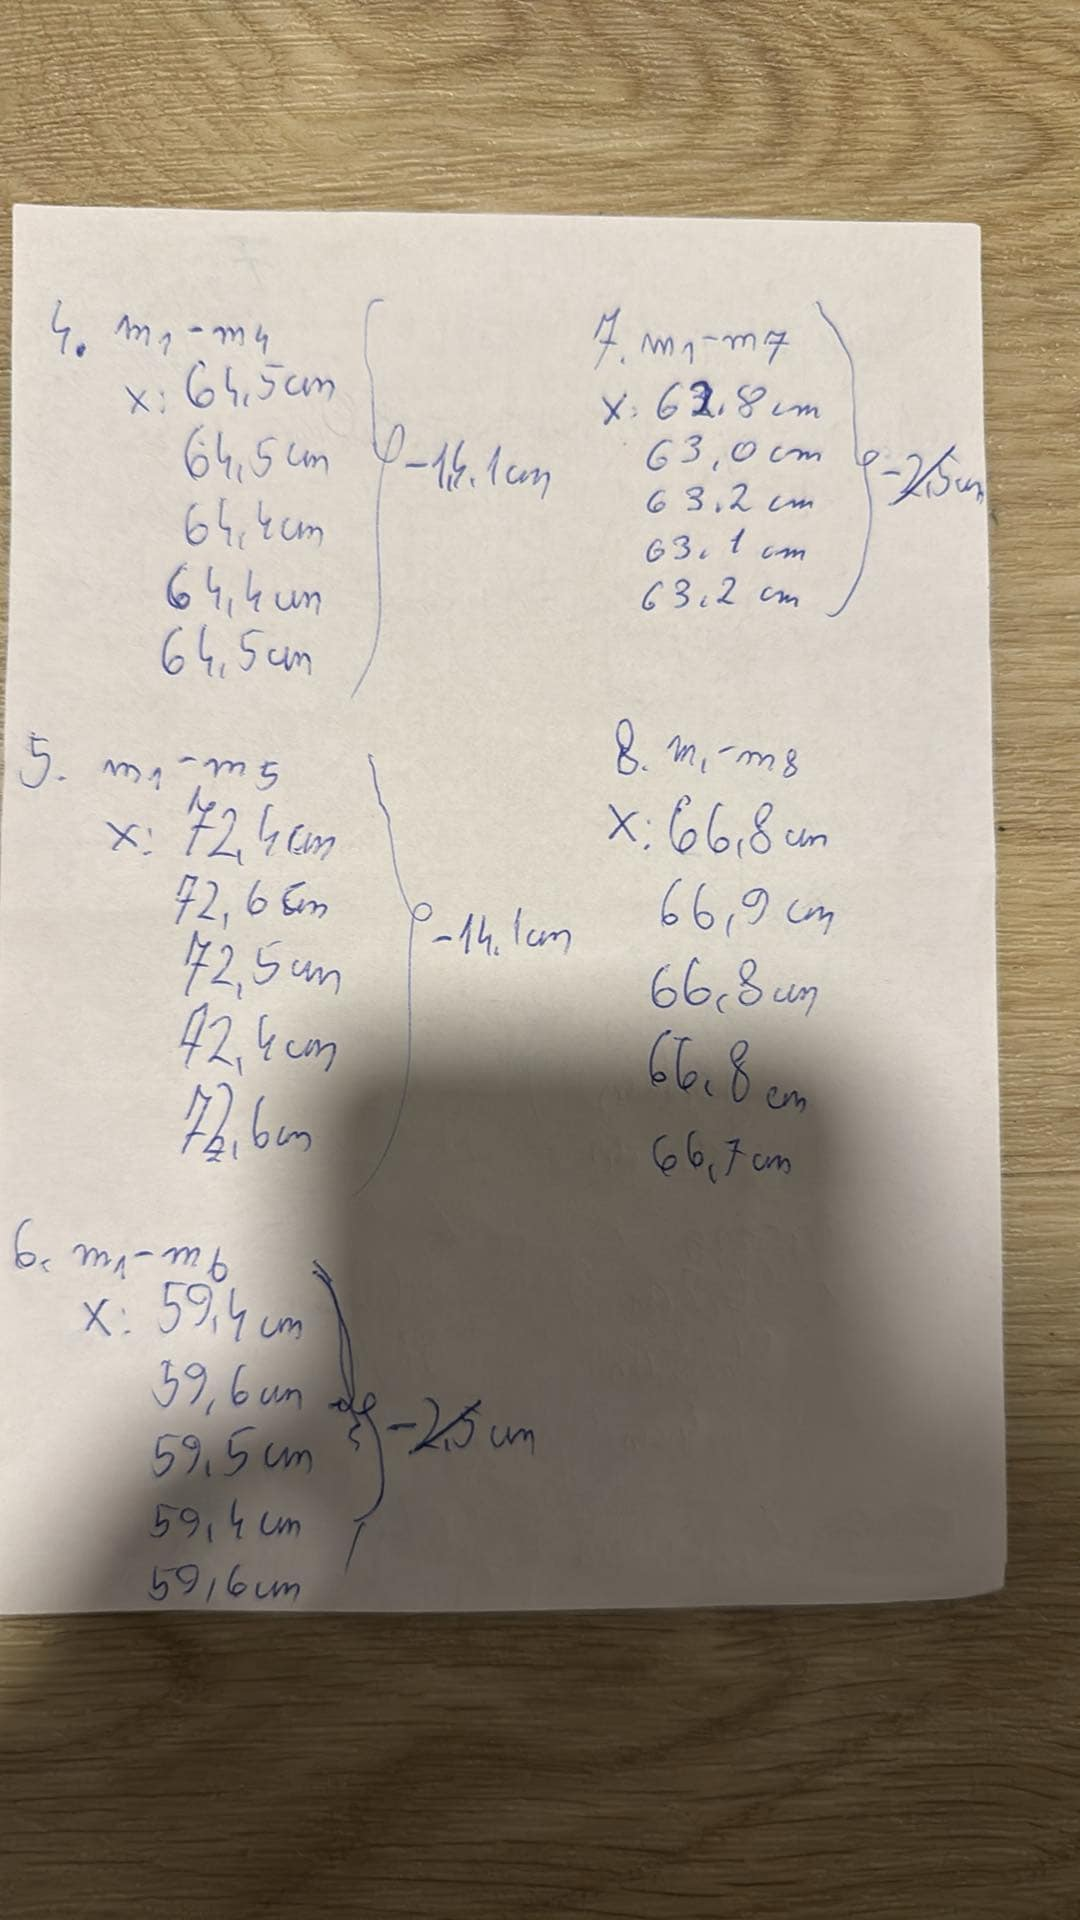
\includegraphics[width=0.5\linewidth]{notes6.jpeg}
\end{figure}
\begin{figure}
    \centering
    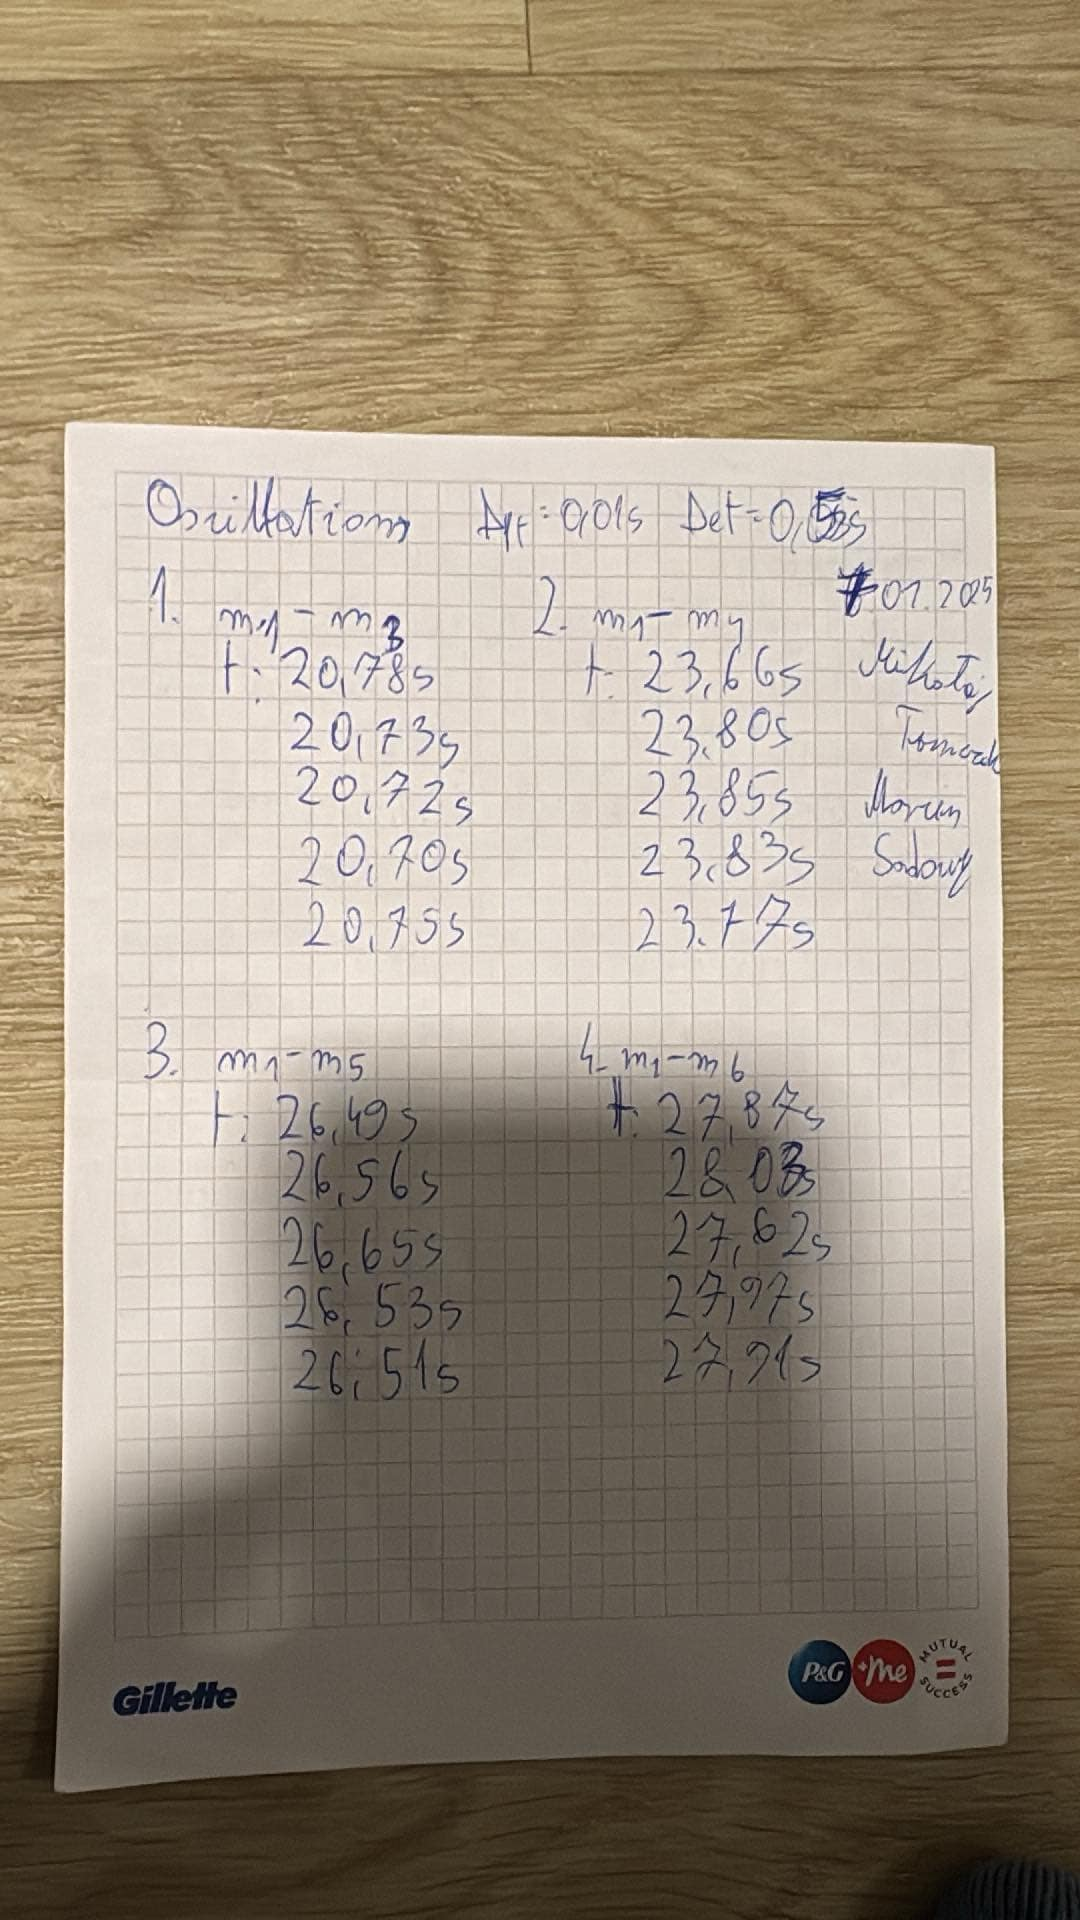
\includegraphics[width=0.5\linewidth]{notes7.jpeg}
\end{figure}
\begin{figure}
    \centering
    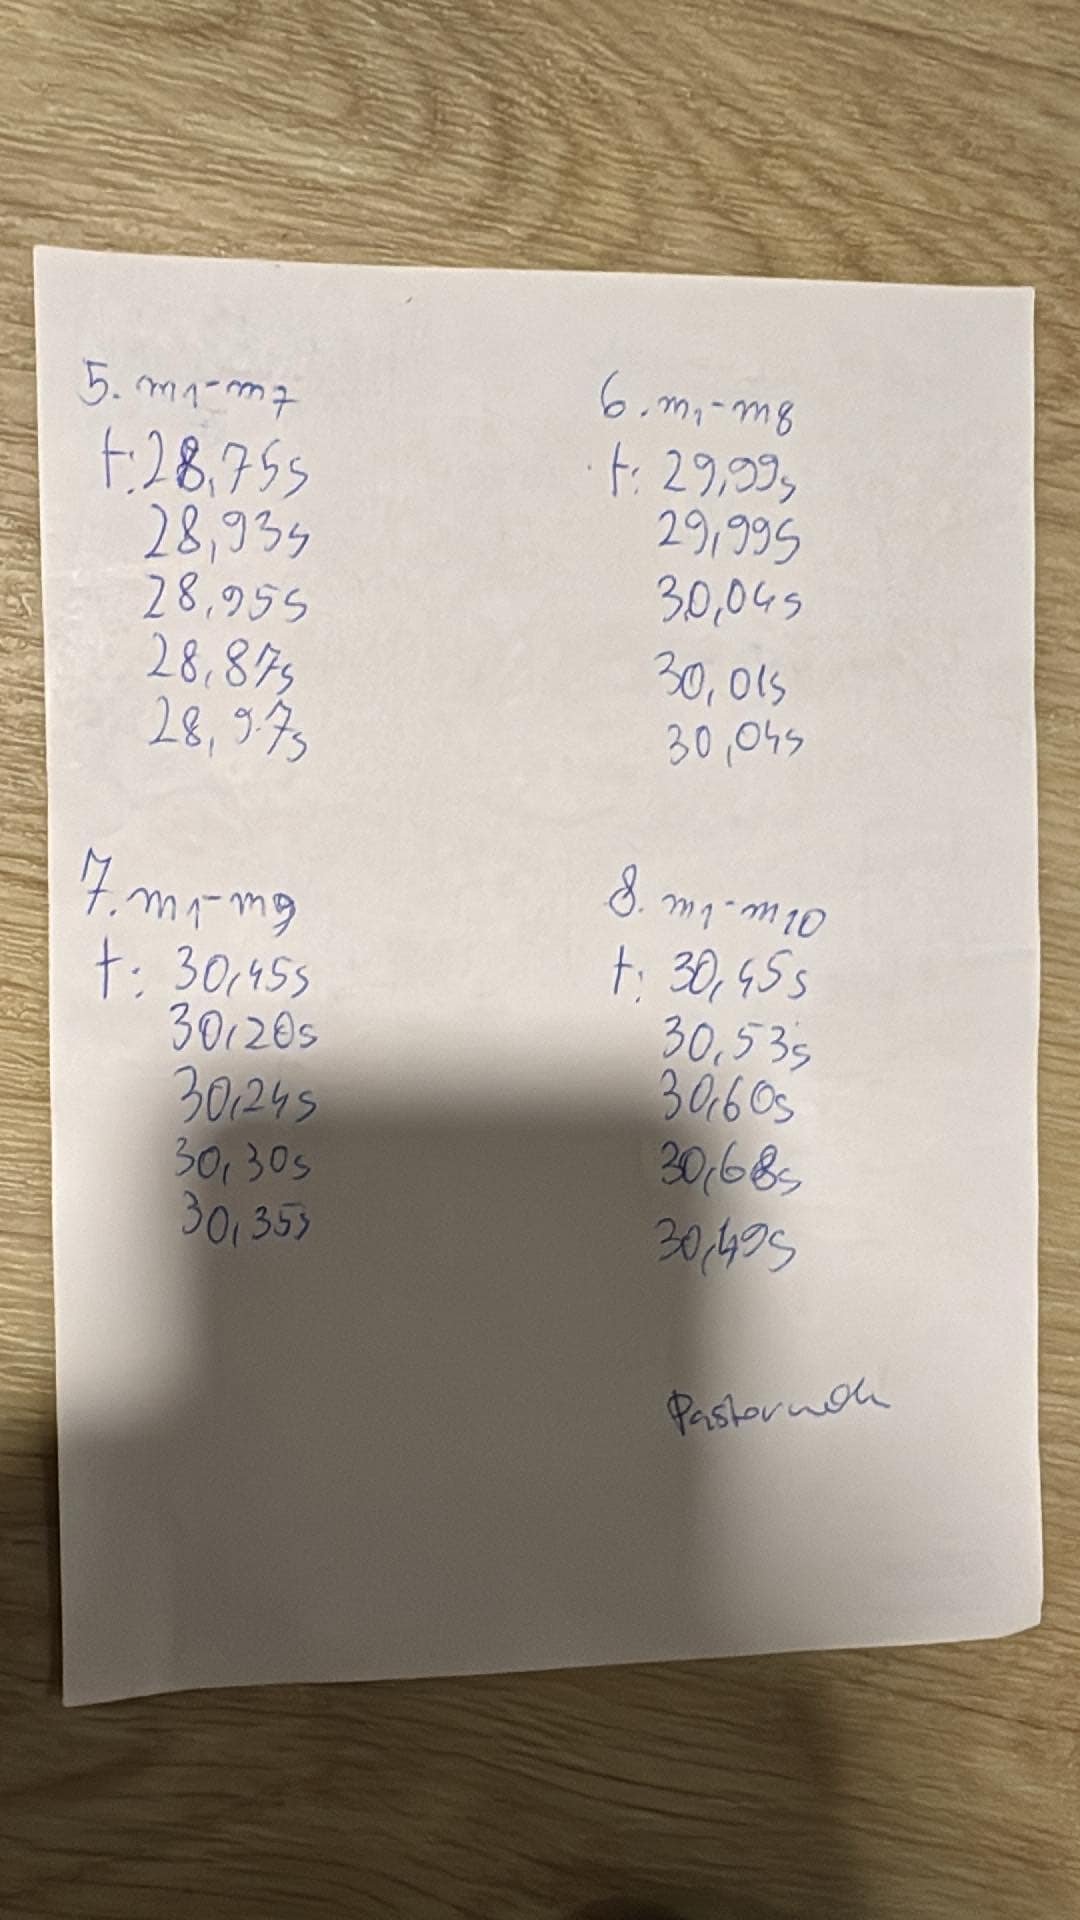
\includegraphics[width=0.5\linewidth]{notes8.jpeg}
\end{figure}
\end{document}
